\section{Design og Implementering}
\label{ch:DesignImplementering}
%%%%%%%%%%%%%%%%%%%%%%%%%%%%
%%%%%%%%%% VBTE %%%%%%%%%%%%
%%%%%%%%%%%%%%%%%%%%%%%%%%%%
\subsection{VBTE}
I dette afsnit beskrives design og implementering af VBTE for både software og hardware. 
\subsubsection{Hardware}
Til VBTE'en er der blevet designet hardware til at styre de to ventiler samt den keramiske ultralydstransmitter og receiver. Hardware er blevet udfærdiget i to dele. Den ene er programeret hardware på PSoC'en, den anden er hardware uden for PSoC'en. Hardware designprocessen til VBTE'en gik igennem 3 faser:
\begin{enumerate}
\item Overordnet design
\item Nedbrydning af blokke
\item Opbygning af design
\end{enumerate}
Gennem disse faser er designet blevet udfærdiget. Fremgangsmåden er anvendt for at overskueligtgøre systemet og lette arbejdet ved at dele systemet op i små dele. På \textit{figur \ref{fig:HWVBTE}} ses det overordnede design af VBTE'en. Der vil i rapporten tages udgangspunkt i ventilkredsen samt receiverdriveren på PSoC'en.
\begin{figure}[H]
\centering
\includegraphics[width = 0.9\textwidth]{billeder/HWVBTE}
\caption{Illustrering af overordnet design af hardware på VBTE.}
\label{fig:HWVBTE}
\end{figure}
\subsubsection{Hardware på PSoC'en}
Hardware opbygget på PSoC'en kunne uden problemer være blevet designet uden for PSoC'en, men PSoC miljøet gør det meget nemt at arbejde med mange forskellige elementer. Der vil i rapporten ligges vægt på transmitterkredsen samt receiverkredsen. På figur \ref{fig:HWVBTE} ses hardware designet på PSoC'en.
\begin{figure}[H]
\centering
\includegraphics[width=0.7\textwidth]{billeder/PSOC_Hardware}
\caption{Hardware på PSoC'en.}
\label{fig:PSOCHW}
\end{figure}
\subsubsection{Transmitterkreds}
Transmitterkredsen står for at sende burst samt at time hvert burst.  Dette opnåes med to clocks, en AND gate, en output pin samt et kontrol register. Transmitterclocken er indstillet til 40kHz da ultralydstransmitteren, ifølge databladet, opererede ved $\SI{40}{kHz}\pm\SI{1}{kHz}$. Clocken er blevet målt på oscilloskop til $\SI{40.3}{kHz}$. Burst kontrolregisteret er anvendt til at AND'e clocken ud på trans\_kontrol pinden.\\
Clock\_dist interruptrutinen sørger for at tælle en variabel op der anvendes i main til at kalde burst funktionen. Dette gøres for at lave et nonblocking delay så andet kan køres på PSoC'en mens en burst er sendt afsted og der afventes detektion.
\subsubsection{Receiverkreds}
Receiverkredsen modtager signalet fra ultralydsreceiveren og omsætter det til en detektion. Dette sker efter følgende opskrift:\\
Løfte signalet $\rightarrow$ Forstærkning $\rightarrow$ Mixning.\\
Signalet bliver løftet på til $\frac{Vdda}{2}$ fordi PSoC'en ikke kan arbejde med værdier under Vssa (GND). Dette gøres ved hjælp af en kondensator, en modstand og en spændingsfølger med $\frac{Vdda}{2}$ på det positive ben.\\
Efter signalet er løftet bliver det forstærket op af en PGA. Efter undersøgelser, hvor der blev sendt burst, er der valgt en forstærkning på 16, da der ca. modtages et signal på $\SI{200}{mV} p-p$.\\
Herefter bliver signalet mixet med $\SI{40}{kHz}$ og filtreret. Efter mixeren giver det, stort set, en DC og summen af de to signaler. Filteret er inbygget i Delta-Sigma ADC'en og har en knækfrekvens ved $\frac{Sample frekvens}{3}$. For at være sikker på at det meste af signalet er kommet over regnes der en opladningstid på filteret til $\SI{1/4}{ms}$. Efter undersøgelser af signalet ind på ADC'en blev en spænding på $\SI{0.3}{V}$.

\subsubsection{Hardware uden for PSoC'en}
Uden for PSoC'en er der lavet 2 hardwareblokke. Disse har til ansvar at omsætte et kontrolsignal til en større spænding over de respektive enheder.
\begin{figure}[H]
	\centering
	\begin{minipage}[b]{0.48\textwidth}\centering
	\includegraphics[width=0.80\textwidth]{billeder/Ventilblok}
	\end{minipage}
	\begin{minipage}[b]{0.48\textwidth}\centering
	\includegraphics[width=0.80\textwidth]{billeder/Transmitterblok}
	\end{minipage}
	\begin{minipage}[t]{0.48\textwidth}
	\caption{Hardwareblok for ventil}
	\label{fig:SMHW1}
	\end{minipage}
	\begin{minipage}[t]{0.48\textwidth}
	\caption{Hardwareblok for transmitteren}
	\label{fig:SMPSOC1}
	\end{minipage}
\end{figure}
\subsubsection{Ventilkreds}
Ventilkredsen får to kontrolsignaler fra PSoC'en og disse skal styre de to ventiler. Ventilerne monteret på kredsen er fra Danfoss og er af modellerne EV210A-1.2 og EV210A-4.5. Disse ventiler drives ved 12V 0.4A. Der er valgt en BD139 transistor til at forstærke signalet op. Denne har en forstærkning mellem 40 og 160 (aflæst fra databladet\footnote{Se bilag/BD139.pdf}). IO's på PSoC'en kan maksimalt trække en strøm på $\SI{4}{mA}$ og det vil i værste tilfælde ikke være nok til at trække ventilerne.\\
Der er derfor lavet en darlington kobling for at mindske belastningen af PSoC'en og for at sikre at der bliver lukket nok op for transistoren. Dette er gjort med en transistor af typen BC547. Transistorne er valgt ud fra pris og tilgængelighed. Der var først valgt en MOSFET IRLZ44n men denne var både for dyr og kunne klare en unødvendig stor effekt. Det smarte ved MOSFET'en er dog at den er spændingsstyret i forhold til de to andre transistorer. 
\subsubsection{Transmitterkreds}
Transmitterkredsen anvender ultralydstranduceren som en højtaler. Denne er koblet over transistoren (Her anvendes også en BD139).\\
\newpage
\begin{figure}[H]
\begin{minipage}[c]{0.45\textwidth}
Via. kontrolsignalet fra PSoC'en, der bliver sendt ud ved $\SI{40}{kHz}$, bliver der sat en spænding over transduceren.\\ 
Forsyningen hertil trækkes fra samme forsyning som ventilkredsen der bliver leveret fra powersuply'en. Ud fra databladet er der aflæst en ohmsk modstand på omtrendt $\SI{10}{k}\Omega$. Derfor kan PSoC'en uden problemer selv trække denne kreds.
\end{minipage}
\begin{minipage}[c]{0.45\textwidth}
\centering
\includegraphics[width = 1\textwidth]{billeder/transmitterkreds}
\caption{Transmitterkreds}
\end{minipage}
\end{figure}
For yderligere detaljer vedrørende hardware på VBTE henvises til \textit{Deltajeret hardware design}.
\subsubsection{Software}
Softwaren til VBTE modulet er blevet designet til at kunne opfylde kravene i kravspecifikationen samt arkitekturen i systemarkitekturen. Den er blevet designet til at passe til hardwaren så den kan kontrollere de enkelte elementer. I designfasen er der blevet udfærdiget et klassediagram samt en statemachine over funktionaliteten. På \textit{figur \ref{fig:VBTEklasse} } ses klassediagramet for VBTE modulets software.
\begin{figure}[H]
\centering
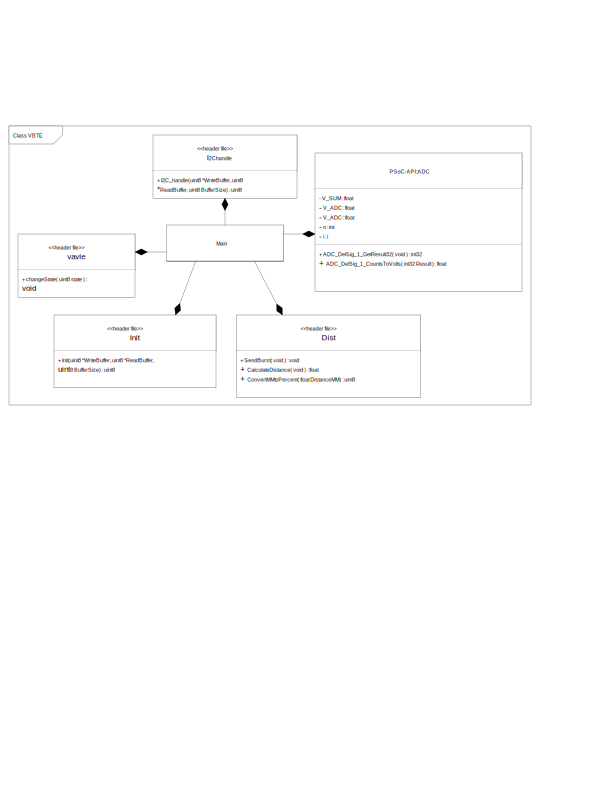
\includegraphics[width=.8\textwidth]{billeder/ClassVBTE}
\label{fig:VBTEklasse}
\caption{Klassediagram over VBTE}
\end{figure}
Selvom softwaren er skrevet i C er der lavet klasser for alle h-filer for at gøre systemet overskueligt. For detaljerede metodebeskriveler henvises til detaljeret software design.\\
For at overskueligtgøre funktionaliteten af softwaren anvendes statemachinediagrammet. Dette viser de forskellige tilstande programmet til enhver til kan befinde sig i.
\begin{figure}[H]
\centering
\includegraphics[width=.8\textwidth]{billeder/STMVBTE}
\caption{Statemachine for VBTE software}
\end{figure}
De forskellige betingelser der skal til for at skifte tilstand vil herefter blive beskrevet. 
%%%%%%%%%%%%%%%%%%%%%%%%%%%%
%%%%%%%%%%% SM %%%%%%%%%%%%%
%%%%%%%%%%%%%%%%%%%%%%%%%%%%
\subsection{SM}
I dette afsnit beskrives design og implementering af SM modulet. SM modulet består af både software og hardware.
\subsubsection{Hardware}
SM modulets hardware består af en konverteringskreds og en PSoC. På PSoC'en er monteret et Kionix KXSC7-2050 accelerometer. Konverteringskredsen anvendes til at sende UART signaler fra PSoC til en KI modulet. Accelerometerets x-akse anvendes til hældningsmålinger for hældningssensorblokken. Designfasen til SM er delt op i 3 faser:
\begin{enumerate}
\item Overordnet design
\item Nedbrydning af blokke
\item Opbygning af design
\end{enumerate}
Denne fremgangsmåde gør det muligt for en udefrakommende at følge med i processen og at kunne implementere modulet så det overholder de krav der er stillet. Ligeledes gør fremgangsmåden det lettere at overskue flere løsninger til hvert problem. på \textit{Figur~\ref{fig:SMHW1}} ses det Overordnede design og på \textit{Figur~\ref{fig:SMPSOC1}} ses PSoC blokken i SM. Der bliver efterfølgende taget udgangspunkt i Hældningssensoren. \\
\begin{figure}[H]
	\centering
	\begin{minipage}[b]{0.48\textwidth}\centering
	\includegraphics[width=0.80\textwidth]{billeder/SMHardware}
	\end{minipage}
	\begin{minipage}[b]{0.48\textwidth}\centering
	\includegraphics[width=0.80\textwidth]{billeder/SMPSoCblock}
	\end{minipage}
	\begin{minipage}[t]{0.48\textwidth}
	\caption{Hardware blok for SM}
	\label{fig:SMHW1}
	\end{minipage}
	\begin{minipage}[t]{0.48\textwidth}
	\caption{PSoC blok for sm}
	\label{fig:SMPSOC1}
	\end{minipage}
\end{figure}
Hældningssensoren består af 2 komponenter: det førnævnte accelerometer samt en DelSig ADC internt i PSoC'en. Valget af accelerometer kommer af at have lavet en række prototyper der ikke mødte vores krav, hvilket accelerometeret i PSoC'en gjorde. Valget af ADC faldt på en DelSig da, den er meget støj immun grundet det indbyggede lavpas filter og har en høj opløsning. Valgte komponenter er illustret på \textit{Figur~\ref{fig:levelsensor}}. ADC konverterer det analoge signal fra, en pin forbundet til, accelerometer til en digital værdi der så senere bliver anvendt i softwaren. For ADC og accelerometerets opsætning se da afsnit \ref{ch:DetajlDesign}~\textit{Detaljeret hardware design} i Bilag.
\begin{figure}[htbp]
	\centering
	\includegraphics[width=0.50\textwidth]{billeder/levelsensor}
	\caption{Hældningssensorens implementering}
	\label{fig:levelsensor}
\end{figure}
\subsubsection{Software}
SM software behandler den konverterede data fra ADC'en samt kommunikation med VBTE og KI modulernerne. Sofwarens udvikling har fulgt de samme faser som hardwaren, hvilket har ført til letforståelig og læselig kode. Softwaren er illustreret på \textit{Figur~\ref{fig:SMKD}}. Der vil efterfølgende blive taget udgangspunkt i et statemachine samt funktionen getFromKI.
\begin{figure}[H]
	\centering
	\includegraphics[width=0.75\textwidth]{billeder/smKlassediagram}
	\caption{Klassediagram for SM}
	\label{fig:SMKD}
\end{figure}
\textbf{SM funktionalitet}\\
Funktionalitet af SM kan bedst beskrives med et state diagram. På \textit{Figur~\ref{fig:SMSTM}} ses  state machine diagrammet for SM modulet. Diagrammet indeholder Automatisk regulering state der beskriver den automatiske regulering i systemet. Den automatiske regulering styres med et flag. Flaget bliver sat når SM opnår forbindelse med KI modulet i 'Afvent' statet. Flaget bliver nulstillet hvis KI sender besked til SM modulet om at det skal termineres, hvorefter SM går tilbage i 'Afvent' statet. Behandlingen af beskeder fra KI i 'Modtag besked fra KI' og 'Send svar til KI' states ses i følgende afsnit \textit{getFromKI}.
\begin{figure}[H]
	\centering
	\includegraphics[width=1\textwidth]{billeder/stmSM}
	\caption{State machine for SM}
	\label{fig:SMSTM}
\end{figure}
\textbf{getFromKI}\\
Funktionen er bedst beskrevet med et flowdiagram:
\begin{figure}[H]
	\centering
	\includegraphics[width=0.75\textwidth]{billeder/getFromKIflowchart}
	\caption{Flowdiagram for funktionen getFromKI}
	\label{fig:gFKIfc}
\end{figure}
Funktionen har til ansvar at kommunikere med KI efter de krav opsat i Kravspecifikation. Hver ACK er relateret til den besked, der er modtaget, så KI modulet ved hvilken besked, SM har modtaget. Dette sikre pålidelig overførsel. 